\chapter{High-Level Architectural Requirements and Documentation}
\label{ch:archreq}

\vspace{-1cm}
\begin{center}
Eduard Hirsch and Thomas Heistracher
\end{center}

\section{About INTERLACE}
The objective of INTERLACE is to use the Abstract State Interaction Machines framework (CoreASIM)\footnote{\url{http://biomicsproject.eu/news/135-icef}} open source output of the FP7 FET project BIOMICS to develop a decentralized transactional and ledger architecture demonstrator for B2B mutual credit.

\section{Introduction and Goals}\label{section-introduction-and-goals}
Currently Sardex uses a well running payment platform which offers solid cooperation and financial transaction facilities. Nevertheless, the architecture has been built using a monolithic centralized approach which is going to be changed. The aim of the platform redesign is to move to decentralized and finally to a completely distributed architecture which is able to scale far beyond the current technically restricted implementations. Figure \ref{decentralizedarchitecture}

\begin{figure}[htbp]
\centering
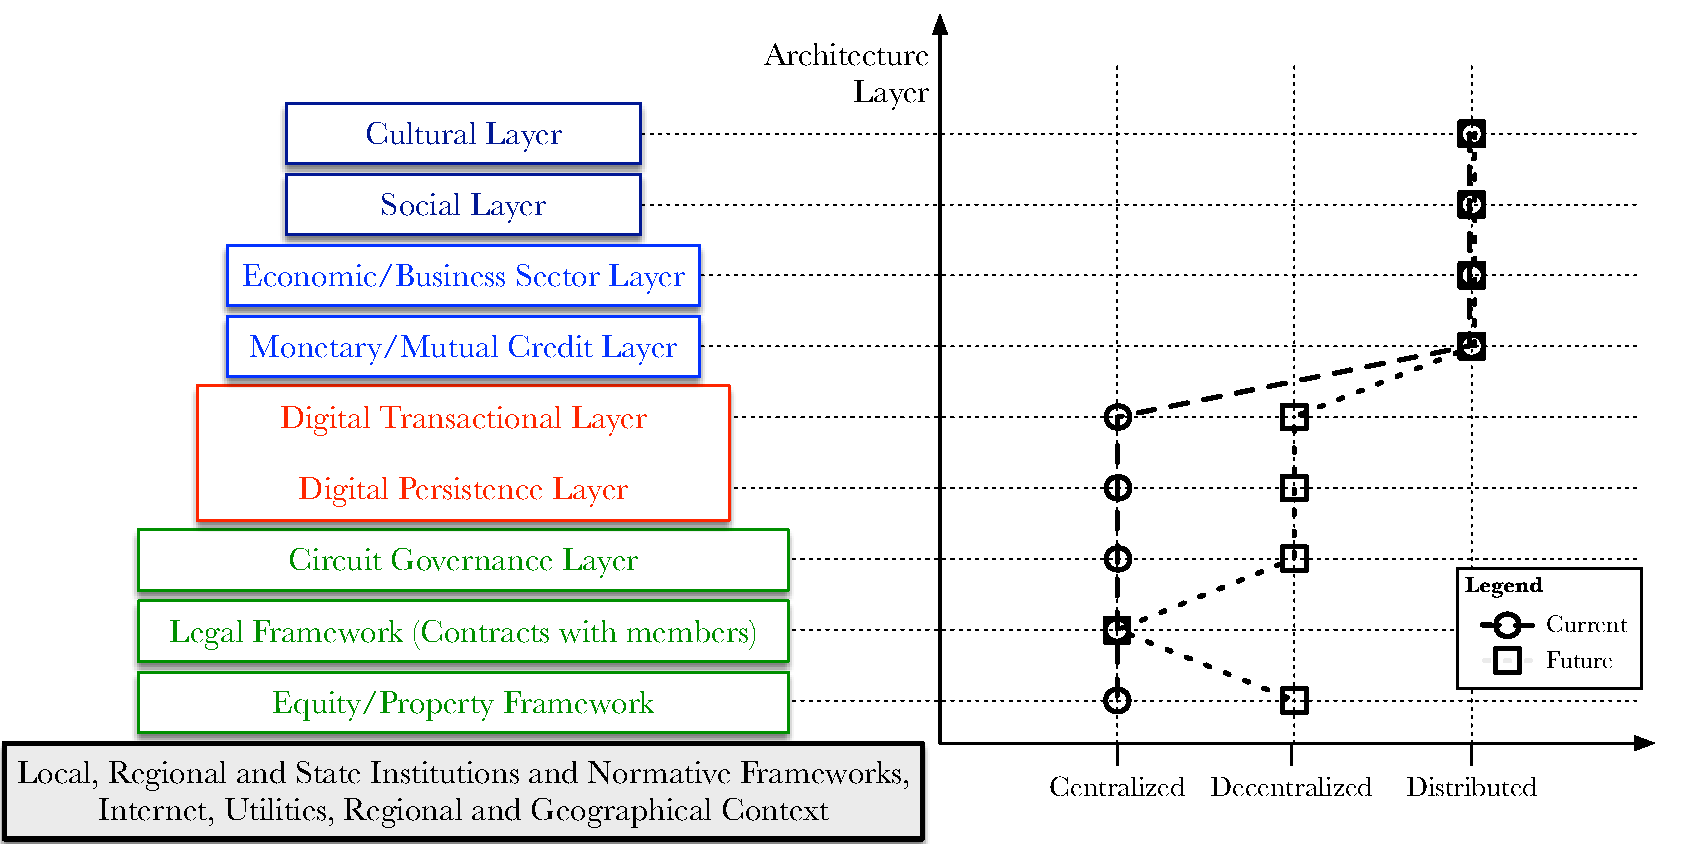
\includegraphics[width=15cm]{Figures/Sardex_Institutional_Structure_V3}
\caption{\small\textbf{Sardex's institutional architecture with current and future decentralization levels}}
\label{decentralizedarchitecture}
\end{figure}

As mentioned above, the business logic will be formulated using the ASM method  \cite{BoergerStaerk2003} to develop executable models of the functional requirements. These models will be implemented in the \textbf{coreASIM} framework,\footnote{\url{http://biomicsproject.eu/news/135-icef}} where they can be validated before implementing them in a production environment (e.g.\ in Java).

The functional requirements addressed in this report cover the core functionalities like credit and debit operations but exclude and intentionally hide implementation details about how transactions are actually processed on the back-end servers. The reason is to enable the ASIMs to communicate directly with the current back-end. After the ASIMs have been verified to execute the current functionalities correctly, the new decentralized/distributed back-end will be developed. Finally, when the new back-end is ready the ASIMs will be changed in order to work with the new logic.

\subsection{Requirements Overview}\label{_requirements_overview}

Next find a list of notes and high level requirements established before and during the first project meetings:

\begin{itemize}

\item[R1] Needs a transaction layer and a persistence layer

\item[R2] Both layers must be extensible and scalable to a (global) distributed architecture, but must start decentralized in their initial (local) implementations

\item[R3] Should be faster than Bitcoin, so a lightweight ledger (fragmented blockchain) approach is preferred

\item[R4] Must be able to support intra-trade and inter-trade between multiple circuits. For example, the different circuits could be:
\begin{itemize}
	\item {different Mutual Credit (MC) circuits (Sardex \& Tibex)}
	\item {different types of networks (MC circuit and Renewable Energy (RE) network)}
\end{itemize}


\item[R5] If possible, reuse existing open source solutions and frameworks, within our own
customized ASM/ASIM framework

\item[R6] Chain code (smart contracts code) should be separate from transaction layer for greater speed and efficiency

\item[R7] Inter-circuit operations must avoid falling under the European PSD2 Directive.
\begin{itemize}
	\item (Giuseppe) This requirement may become obsolete if we use Stripe (\url{https://stripe.com/docs}) and Telegram (\url{https://telegram.org/blog/payments})
	\item (Giuseppe) Note: currently there is one cloud instance of the DB. Inter-circuit payments are within the same DB (Cyclos 4) and are movements between different user groups. In future we may mirror or reproduce the network in a distributed manner and then start a node at least for each local network
	\item (Paolo) The requirement of a single point of legal liability remains even if we use
Stripe. Buyer and seller must each have a contract with the same entity (Sardex
S.p.A.)
\end{itemize}


\item[R8] The Sardex blockchain should not have a native token: this is in order to separate unit of
account and medium of exchange from the operation of platform (i.e. no mining, as in Bitcoin)
and avoid seignorage (as in Ripple/XRP)
\begin{itemize}
	\item (Giuseppe) I meant it as a proposal, I am not sure the ecosystem couldn’t grow faster and healthier if a proper social protocol and seignorage would become possible (à la distributed XRP)
	\item (Paolo) Anything that strengthens the store of value perception of the currency will make our job more difficult. I would stay away from it.
	\item (Giuseppe) The rationale would be that a store of value is useful when there is no fiat or insurance that can save peers from the pain/cost of other peers defaulting
\end{itemize}


\item[R9] Smart contracts code should not be Turing-complete (this requirement might be deleted)
\begin{itemize}
	\item (Giuseppe) The turing completeness gives attackers on a publicly deployed network larger attack surfaces:
	\begin{itemize}
		\item \url{https://www.reddit.com/r/btc/comments/4p0gq3/why_turingcomplete_smart_contracts_are_doomed/}
		\item \url{https://hackernoon.com/smart-contracts-turing-completeness-reality-3eb897996621}
		\item \href{https://www.quora.com/How-is-Tezos-different-from-Ethereum}{Tezos}
	\end{itemize}

	\item (Egon) The undecidability of Turing-complete languages does not prevent the ability to prove specific properties of specific programs. In the ASM methodology, provability is refined along with the specifications as part of the iterative refinement process, down to the actual code.
\end{itemize}


\item[R10] Whatever solution we adopt, it should be compatible with the emerging InterLedger
standard, which will play a role similar to the Internet in allowing different payment
systems to interoperate. InterLedger has been approved by W3C.
\begin{itemize}
	\item (Giuseppe) Not 100% sure we need to take it into account since it mainly offers escrow functions https://interledger.org/rfcs/0001-interledger-architecture/
	\item (Giuseppe) W3C WEB-PAYMENTS STANDARD API ----- super relevant \url{https://www.w3.org/TR/payment-request/}
\end{itemize}


\item[R11] Platform must involve the current regional MC systems and a global reward and digital asset system called Proximity and whose unit of account is called $\pi $ (Pi)

\item[R12] {Proximity involves a reward points system whereby πs are awarded to users on the basis of behaviour that is beneficial for (their local) MC system. Gaining πs translates into the ability to trade farther away from the user’s geographical location. Upon reaching a certain threshold, the user is allowed to trade inter-circuit. There is a π cost associated with inter-circuit trade (see R13). There is also a commission in Euro on all inter-circuit trades (e.g. 2\%).}

\item[R13] A likely scenario for the fee in πs is NOT to tie it to the transaction amount but, RATHER, to use it as a mechanism to offset the inter-circuit trade balances, i.e. in effect as a customs duty. Rather than just a cost, however, the fact that πs can be given as a reward as well as charged as duty means that as an instrument to shape the (inter-circuit) market they should be more
effective than mere protectionist policy.

\item[R14] After some discussion, it became clear that the new platform architecture should be closed, i.e. ‘permissioned’, both for the regional networks and for Proximity:
\begin{itemize}
	\item Open (permissionless) DLT networks like Ripple/XRP could not prevent external actors
from speculating on Sardex digital assets like π
	\item Private (permissioned) DLTs like Chain Core/Ivy (compatible with PSD2) are preferred
\end{itemize}


\item[R15] State objects must be immutable: this is important in order to prevent people going back on their commitments, for example the max number of credits they will accept (there are examples of blockchains whose previous blocks have been modified - Ethereum DAO Hack)

\end{itemize}

Detailed functional requirements can be found in the chapter \ref{ch:funreq}

\subsection{Quality Goals}\label{_quality_goals}

\subsection{Stakeholders and their roles}\label{_stakeholders}

\begin{itemize}
	\item B ... Business
	\item C ... Customer
	\item E ... Employee	
\end{itemize}

\begin{longtable}[]{@{}lll@{}}
\toprule
\begin{minipage}[b]{0.18\columnwidth}\raggedright\strut
Role/Name\strut
\end{minipage} & \begin{minipage}[b]{0.37\columnwidth}\raggedright\strut
Contact\strut
\end{minipage} & \begin{minipage}[b]{0.37\columnwidth}\raggedright\strut
Expectations\strut
\end{minipage}\tabularnewline
\midrule
\endhead
\begin{minipage}[t]{0.18\columnwidth}B2B \end{minipage} &
\begin{minipage}[t]{0.37\columnwidth}Participating Companies \end{minipage} &
\begin{minipage}[t]{0.37\columnwidth}Business to business transactions and interaction\end{minipage}
\tabularnewline
\tabularnewline
\begin{minipage}[t]{0.18\columnwidth}B2E \end{minipage} &
\begin{minipage}[t]{0.37\columnwidth}Employees \end{minipage} &
\begin{minipage}[t]{0.37\columnwidth}Payments of Employees\end{minipage}
\tabularnewline
\tabularnewline
\begin{minipage}[t]{0.18\columnwidth}B2C \end{minipage} &
\begin{minipage}[t]{0.37\columnwidth}Normal Customer \end{minipage} &
\begin{minipage}[t]{0.37\columnwidth}Payments to Participating Companies\end{minipage}
\tabularnewline
\tabularnewline
\begin{minipage}[t]{0.18\columnwidth}Sardex-Admin \end{minipage} &
\begin{minipage}[t]{0.37\columnwidth}Sardex Employee \end{minipage} &
\begin{minipage}[t]{0.37\columnwidth}Configuring and maintaining the infrastructure\end{minipage}
\tabularnewline
\tabularnewline
\begin{minipage}[t]{0.18\columnwidth}Sardex-Manager \end{minipage} &
\begin{minipage}[t]{0.37\columnwidth}Sardex Employee \end{minipage} &
\begin{minipage}[t]{0.37\columnwidth}Running evaluations and managing the cooperation platform \end{minipage}
\tabularnewline


\bottomrule
\end{longtable}

\section{Solution Strategy}\label{section-solution-strategy}

The strategy of how to get from a monolithic working implementation to a decentralized and later a fully fledged distributed ledger application, as during introduction mentioned, will be done over the use of Abstract State Machines (ASMs). They do not just offer defining functional requirements for the purpose of documentation (found in Chapter \ref{ch:funreq}) but also are able to directly derive a working implementation.

Unfortunately plain ASMs have a quite narrow scope and are working only in their own scope and have no shared states. So it is not possible with them creating a decentralized or a even fully distributed environment where the new implementation can work in.

The solution for the INTERLACE project is offered by the BIOMICS project which had as outcome a special extension of the ASMs named Abstract Interaction Machines (ASIMs) and a corresponding runtime environment called Interaction Computing Execution Framework (ICEF) \footnote{\url{https://github.com/biomics/icef}}.

\textbf{Quoting the ICEF webpage:}
\begin{quote}
"This framework extends the original CoreASM modelling and execution framework to enable the specification and execution of \textbf{distributed and concurrent} ASMs.

The ICEF was developed in the STREP project BIOMICS which was financed by the European Comission in FP7 from October 1st, 2012 until March 31st, 2016.

ICEF enables asynchronous execution of ASMs. It uses and enhances the CoreASM execution engine to support communicating and interacting ASMs: CoreASIMs. Further, ICEF replaces ASM with BSL which offers additional language primitives specifically designed to define the beahviour of biochemical systems.

This code introduces a restful API to control the BIOMICS wrapper (brapper) which can host several CoreASIM instances and enables networked CoreASIM. It also introduces a manager which orchestrates several ASIMs to allow the execution of interaction computing simulations."
\end{quote}

Although the additional language primitives offered by ICEF might not be needed the coreASIM implementation will be crucial for realizing the INTERLACE strategy.

\subsection{Strategy Steps}\label{subsection-strategy-steps}

\begin{enumerate}

	\item Defining the functional requirements using the ASMs formal description language.
	\item Translating the formal description to a working demo environment using ICEF/coreASIM.
	\item Brining the coreASIM business logic together with the real world. That means to use the interaction capabilities of the framework to connect it to legacy application.
	\item Test if the application still works and the translation to coreASIM has been working.
	\item Translating the coreASIM implementation to a "real-world" application by creating e.g. a JAVA. application.
	\item Developing a verifying strategy and verify the implemented "real-world" application.
	\item Change the ASIM models to work in a distributed environment.
	\item Adapt ASIM interfaces.
	\item Adapt the "real-world" version.
	\item Implement the new back-end logic using Open Source frameworks.
	\item Test/Validate the new application against the new back-end.
 
\end{enumerate}
	
%\section{Architecture
%Constraints}\label{section-architecture-constraints}

%\section{System Scope and
%Context}\label{section-system-scope-and-context}

%\subsection{Business Context}\label{_business_context}

%\textbf{\textless{}Diagram or Table\textgreater{}}

%\textbf{\textless{}optionally: Explanation of external domain
%interfaces\textgreater{}}

%\subsection{Technical Context}\label{_technical_context}

%\textbf{\textless{}Diagram or Table\textgreater{}}

%\textbf{\textless{}optionally: Explanation of technical
%interfaces\textgreater{}}

%\textbf{\textless{}Mapping Input/Output to Channels\textgreater{}}

%\section{Solution Strategy}\label{section-solution-strategy}

%\section{Building Block View}\label{section-building-block-view}

%\subsection{Whitebox Overall System}\label{_whitebox_overall_system}

%\emph{\textbf{\textless{}Overview Diagram\textgreater{}}}

%\begin{description}
%\item[Motivation]
%\emph{\textless{}text explanation\textgreater{}}
%\item[Contained Building Blocks]
%\emph{\textless{}Description of contained building block (black
%boxes)\textgreater{}}
%\item[Important Interfaces]
%\emph{\textless{}Description of important interfaces\textgreater{}}
%\end{description}

%\subsubsection{\textless{}Name black box
%1\textgreater{}}\label{__name_black_box_1}

%\emph{\textless{}Purpose/Responsibility\textgreater{}}

%\emph{\textless{}Interface(s)\textgreater{}}

%\emph{\textless{}(Optional) Quality/Performance
%Characteristics\textgreater{}}

%\emph{\textless{}(Optional) Directory/File Location\textgreater{}}

%\emph{\textless{}(Optional) Fulfilled Requirements\textgreater{}}

%\emph{\textless{}(optional) Open Issues/Problems/Risks\textgreater{}}

%\subsubsection{\textless{}Name black box
%2\textgreater{}}\label{__name_black_box_2}

%\emph{\textless{}black box template\textgreater{}}

%\subsubsection{\textless{}Name black box
%n\textgreater{}}\label{__name_black_box_n}

%\emph{\textless{}black box template\textgreater{}}

%\subsubsection{\textless{}Name interface
%1\textgreater{}}\label{__name_interface_1}

%\ldots{}

%\subsubsection{\textless{}Name interface
%m\textgreater{}}\label{__name_interface_m}

%\subsection{Level 2}\label{_level_2}

%\subsubsection{\texorpdfstring{White Box \emph{\textless{}building block
%1\textgreater{}}}{White Box \textless{}building block 1\textgreater{}}}\label{_white_box_emphasis_building_block_1_emphasis}

%\emph{\textless{}white box template\textgreater{}}

%\subsubsection{\texorpdfstring{White Box \emph{\textless{}building block
%2\textgreater{}}}{White Box \textless{}building block 2\textgreater{}}}\label{_white_box_emphasis_building_block_2_emphasis}

%\emph{\textless{}white box template\textgreater{}}

%\ldots{}

%\subsubsection{\texorpdfstring{White Box \emph{\textless{}building block
%m\textgreater{}}}{White Box \textless{}building block m\textgreater{}}}\label{_white_box_emphasis_building_block_m_emphasis}

%\emph{\textless{}white box template\textgreater{}}

%\subsection{Level 3}\label{_level_3}

%\subsubsection{White Box \textless{}\_building block
%x.1\_\textgreater{}}\label{_white_box_building_block_x_1}

%\emph{\textless{}white box template\textgreater{}}

%\subsubsection{White Box \textless{}\_building block
%x.2\_\textgreater{}}\label{_white_box_building_block_x_2}

%\emph{\textless{}white box template\textgreater{}}

%\subsubsection{White Box \textless{}\_building block
%y.1\_\textgreater{}}\label{_white_box_building_block_y_1}

%\emph{\textless{}white box template\textgreater{}}

%\section{Runtime View}\label{section-runtime-view}

%\subsection{\textless{}Runtime Scenario
%1\textgreater{}}\label{__runtime_scenario_1}

%\begin{itemize}
%\item
%  \emph{\textless{}insert runtime diagram or textual description of the
%  scenario\textgreater{}}
%\item
%  \emph{\textless{}insert description of the notable aspects of the
%  interactions between the building block instances depicted in this
%  diagram.\textgreater{}}
%\end{itemize}

%\subsection{\textless{}Runtime Scenario
%2\textgreater{}}\label{__runtime_scenario_2}

%\subsection{\ldots{}}\label{_}

%\subsection{\textless{}Runtime Scenario
%n\textgreater{}}\label{__runtime_scenario_n}

%\section{Deployment View}\label{section-deployment-view}

%\subsection{Infrastructure Level 1}\label{_infrastructure_level_1}

%\emph{\textbf{\textless{}Overview Diagram\textgreater{}}}

%\begin{description}
%\item[Motivation]
%\emph{\textless{}explanation in text form\textgreater{}}
%\item[Quality and/or Performance Features]
%\emph{\textless{}explanation in text form\textgreater{}}
%\item[Mapping of Building Blocks to Infrastructure]
%\emph{\textless{}description of the mapping\textgreater{}}
%\end{description}

%\subsection{Infrastructure Level 2}\label{_infrastructure_level_2}

%\subsubsection{\texorpdfstring{\emph{\textless{}Infrastructure Element
%1\textgreater{}}}{\textless{}Infrastructure Element 1\textgreater{}}}\label{__emphasis_infrastructure_element_1_emphasis}

%\emph{\textless{}diagram + explanation\textgreater{}}

%\subsubsection{\texorpdfstring{\emph{\textless{}Infrastructure Element
%2\textgreater{}}}{\textless{}Infrastructure Element 2\textgreater{}}}\label{__emphasis_infrastructure_element_2_emphasis}

%\emph{\textless{}diagram + explanation\textgreater{}}

%\ldots{}

%\subsubsection{\texorpdfstring{\emph{\textless{}Infrastructure Element
%n\textgreater{}}}{\textless{}Infrastructure Element n\textgreater{}}}\label{__emphasis_infrastructure_element_n_emphasis}

%\emph{\textless{}diagram + explanation\textgreater{}}

%\section{Cross-cutting Concepts}\label{section-concepts}

%\subsection{\texorpdfstring{\emph{\textless{}Concept
%1\textgreater{}}}{\textless{}Concept 1\textgreater{}}}\label{__emphasis_concept_1_emphasis}

%\emph{\textless{}explanation\textgreater{}}

%\subsection{\texorpdfstring{\emph{\textless{}Concept
%2\textgreater{}}}{\textless{}Concept 2\textgreater{}}}\label{__emphasis_concept_2_emphasis}

%\emph{\textless{}explanation\textgreater{}}

%\ldots{}

%\subsection{\texorpdfstring{\emph{\textless{}Concept
%n\textgreater{}}}{\textless{}Concept n\textgreater{}}}\label{__emphasis_concept_n_emphasis}

%\emph{\textless{}explanation\textgreater{}}

%\section{Design Decisions}\label{section-design-decisions}

%\section{Quality Requirements}\label{section-quality-scenarios}

%\subsection{Quality Tree}\label{_quality_tree}

%\subsection{Quality Scenarios}\label{_quality_scenarios}

\section{Risks and Technical Debts}\label{section-technical-risks}

\section{Glossary}\label{section-glossary}

\begin{longtable}[]{@{}ll@{}}
\toprule
\begin{minipage}[b]{0.47\columnwidth}\raggedright\strut
Term\strut
\end{minipage} & \begin{minipage}[b]{0.47\columnwidth}\raggedright\strut
Definition\strut
\end{minipage}\tabularnewline
\midrule
\endhead
\begin{minipage}[t]{0.47\columnwidth}\raggedright\strut
\textless{}Term-1\textgreater{}\strut
\end{minipage} & \begin{minipage}[t]{0.47\columnwidth}\raggedright\strut
\textless{}definition-1\textgreater{}\strut
\end{minipage}\tabularnewline
\begin{minipage}[t]{0.47\columnwidth}\raggedright\strut
\textless{}Term-2\textgreater{}\strut
\end{minipage} & \begin{minipage}[t]{0.47\columnwidth}\raggedright\strut
\textless{}definition-2\textgreater{}\strut
\end{minipage}\tabularnewline
\bottomrule
\end{longtable}
